\documentclass[11pt]{article}
\usepackage[margin=1in]{geometry}
\usepackage{amsmath,amssymb}
\usepackage{booktabs}
\usepackage{algorithm}
\usepackage{algpseudocode}
\usepackage{tikz}
\usepackage[hidelinks]{hyperref}

\newcommand{\vect}[1]{\mathbf{#1}}
\newcommand{\edot}{\dot{\varepsilon}}
\newcommand{\dd}{\,\mathrm{d}}
\newcommand{\Hint}{\mathcal{H}}
\newcommand{\Bint}{\mathcal{B}}
\renewcommand{\algorithmicrequire}{\textbf{Input:}}
\renewcommand{\algorithmicensure}{\textbf{Output:}}

\title{A Conservative Vertex-Centred Arbitrary Lagrangian--Eulerian Method\\
for Plate-Scale Lithospheric Deformation\\
with Evolving Ridges, Transforms, Trenches and Slab Pull}
\author{}
\date{}

\begin{document}
\maketitle

\begin{abstract}
We describe a numerical method for the large-scale horizontal deformation of continental and oceanic lithosphere, treated as a thin, isostatically compensated, power-law viscous sheet resting on a mantle that exerts basal drag. Each column of lithosphere is described by its crustal thickness, crustal density, heat deficit and integrity. A heat-balance integral closure makes the heat deficit evolve by conductive cooling without an explicit age field, so seafloor subsidence, ridge push and plate strengthening follow from the column physics. All state lives on moving markers, each owning the integrals of these quantities over its median dual cell. A constrained Delaunay triangulation of the markers carries no state and supports a linear finite element solution of the depth-integrated force balance. Plate boundaries are represented as seams of split markers, so that ridges, transforms and trenches coincide exactly with cell boundaries. Ridges create lithosphere; trenches consume it into a per-node slab reservoir whose negative buoyancy, less mantle drag, pulls on the subducting plate. Seams are not prescribed: they open where neighbouring columns slide past one another, become trenches where negatively buoyant lithosphere converges on them, become ridges where thin lithosphere diverges, lose their slab when positively buoyant lithosphere arrives at a trench, and heal where they stop slipping. Plates are simply the regions that seams enclose. Basal drag depends on local lithospheric thickness, so thick keels couple more strongly to the mantle than young, thin plates. Mass moves between cells only by fluxes through shared faces, so all budgets close to round-off. The method is a vertex-centred control volume finite element method (CVFEM) in arbitrary Lagrangian--Eulerian (ALE) form, and we include notes on implementing it in a web browser with WebGPU.
\end{abstract}

\tableofcontents

%======================================================================
\section{Physical model}
%======================================================================

\subsection{Assumptions}
\begin{enumerate}
\item \textbf{Thin sheet.} Horizontal length scales greatly exceed lithospheric thickness, and horizontal velocity $\vect{u}(x,y,t)$ is independent of depth: a vertical line through the lithosphere stays vertical. Consequently, horizontal divergence thins or thickens every layer of a column by the same factor.
\item \textbf{Isostasy.} Every column is in local hydrostatic equilibrium above a common compensation depth. Depressions below sea level fill with water.
\item \textbf{Overdamped flow.} Inertia is negligible; viscous, drag and boundary forces balance buoyancy forces at every instant.
\item \textbf{Column structure.} A column consists of a crust of thickness $h$ and uniform compositional density $\rho_c$, over mantle of density $\rho_m$. Compositional densities are quoted at mantle temperature $T_m$; the equivalent surface-temperature density is $\rho(1+\alpha\Delta T)$.
\item \textbf{Thermal structure.} The temperature deficit $T_m-T$ has the self-similar half-space (error-function) profile. Thermal contraction is $\rho_m\alpha(T_m-T)$ throughout the column, including the crust (an error of order $\rho_c/\rho_m-1$ within the crust).
\item \textbf{Rheology.} Incompressible power-law creep, with depth-integrated strength depending on crustal thickness, thermal thickness and a scalar integrity $s\in[0,1]$.
\item \textbf{Basal drag} linear in velocity, in the frame of the underlying mantle, with a coefficient $\beta\ge0$ that depends on the local lithospheric thickness (Section~\ref{sec:drag}).
\item \textbf{Plate boundaries} are seams across which velocity may jump. Their positions move with the flow, and their existence and type follow local rules on the column state and the relative motion across them (Section~\ref{sec:lifecycle}).
\end{enumerate}
The model is planar. It excludes elastic flexure, depth-dependent flow such as lower-crustal channel flow, erosion and sedimentation, radiogenic heating, and three-dimensional slab dynamics, which are replaced by a reservoir model (Section~\ref{sec:slabmodel}).

\subsection{Column state}
Each column carries four quantities per unit area:
\begin{center}
\begin{tabular}{@{}lll@{}}
\toprule
Symbol & Meaning & Units\\
\midrule
$h$ & crustal thickness & m\\
$\rho_c$ & crustal compositional density (at $T_m$) & kg\,m$^{-3}$\\
$\Theta=\int_0^\infty (T_m-T)\dd\zeta$ & heat deficit ($\zeta$ = depth below solid surface) & K\,m\\
$s$ & integrity (1 intact, 0 fully damaged) & --\\
\bottomrule
\end{tabular}
\end{center}

\subsection{Thermal closure}
\label{sec:thermal}
For the half-space profile $T_m-T=\Delta T\,\operatorname{erfc}(\zeta/\delta)$ with $\Delta T=T_m-T_s$ and $\delta=2\sqrt{\kappa\tau}$, the heat deficit and its first moment are
\begin{equation}
  \Theta = \frac{\Delta T\,\delta}{\sqrt\pi},\qquad
  M_1 \equiv \int_0^\infty \zeta\,(T_m-T)\dd\zeta = \frac{\Delta T\,\delta^2}{4} = \frac{\pi\,\Theta^2}{4\,\Delta T}.
  \label{eq:moments}
\end{equation}
The surface heat flow $k\Delta T/\sqrt{\pi\kappa\tau}$ can be written in terms of $\Theta$ alone, giving the cooling law, following the material,
\begin{equation}
  \frac{D\Theta}{Dt} = \frac{2\kappa\,\Delta T^2}{\pi\,\Theta} - \frac{q_b}{\rho_m c_p},
  \label{eq:cooling}
\end{equation}
where $\kappa$ is thermal diffusivity and $q_b\ge0$ an optional basal heat flux that makes old lithosphere approach a steady thickness (as in plate-cooling models); with $q_b=0$ the law is pure half-space cooling.

Two properties make the closure exact, not merely plausible, for $q_b=0$:
\begin{itemize}
\item For lithosphere created at $\Theta=0$ and carried rigidly, integrating~\eqref{eq:cooling} gives $\Theta=2\Delta T\sqrt{\kappa\tau/\pi}$, the exact half-space result at age $\tau$.
\item Under depth-uniform horizontal divergence (Assumption 1), the profile is compressed or stretched uniformly in depth. A vertically rescaled error-function profile is again an error-function profile, of a different effective age, so the closure remains exact through any history of stretching or shortening the sheet can represent.
\end{itemize}
Without an age variable, the cooling law is integrated exactly over a step of length $\Delta t$ (for $q_b=0$):
\begin{equation}
  \Theta(t+\Delta t) = \sqrt{\Theta(t)^2 + 4\kappa\,\Delta T^2\,\Delta t/\pi},
  \label{eq:coolexact}
\end{equation}
which removes the apparent singularity at $\Theta=0$.

\subsection{Isostasy and elevation}
Let $z$ point upward from sea level, let $e$ be the elevation of the solid surface, and let $D$ be a compensation depth deeper than every column. Equal pressure at $z=-D$ under all columns gives the ``dry'' elevation
\begin{equation}
  e^\ast = e_0 + h\left(1-\frac{\rho_c}{\rho_m}\right) - \alpha\,\Theta,
\end{equation}
and the actual elevation, accounting for water loading below sea level,
\begin{equation}
  e = \begin{cases} e^\ast & e^\ast\ge0,\\[2pt] \dfrac{\rho_m}{\rho_m-\rho_w}\,e^\ast & e^\ast<0.\end{cases}
  \label{eq:elev}
\end{equation}
The constant $e_0$ is fixed by requiring a zero-age ridge column ($h=h_{oc}$, $\rho_c=\rho_{oc}$, $\Theta=0$) to sit at a chosen ridge depth $e_r<0$:
\begin{equation}
  e_0 = \frac{\rho_m-\rho_w}{\rho_m}\,e_r - h_{oc}\left(1-\frac{\rho_{oc}}{\rho_m}\right).
\end{equation}
For oceanic lithosphere this reproduces subsidence $\rho_m\alpha\Theta/(\rho_m-\rho_w)\propto\sqrt{\tau}$.

\subsection{Gravitational potential energy}
The driving potential is the depth-integrated lithostatic pressure, equivalently the gravitational potential energy (GPE) per unit area measured from the compensation depth,
\begin{equation}
  \Phi = \int_{-D}^{z_{\mathrm{top}}} P(z)\dd z = g\int_{-D}^{z_{\mathrm{top}}}\rho(z)\,(z+D)\dd z,
  \qquad z_{\mathrm{top}}=\max(e,0).
\end{equation}
For the column above, this evaluates in closed form as the sum of four contributions:
\begin{align}
  \Phi(h,\rho_c,\Theta) = g\Big[\;&\rho_w\,(-e)_+\,\big(D+\tfrac12 e\big) && \text{water}\nonumber\\
  &+\rho_c\,h\,\big(e-\tfrac12h+D\big) && \text{crust}\nonumber\\
  &+\tfrac12\rho_m\,(e-h+D)^2 && \text{mantle}\nonumber\\
  &+\rho_m\alpha\,\big((e+D)\,\Theta - M_1(\Theta)\big)\;\Big] && \text{thermal contraction},
  \label{eq:phi}
\end{align}
with $e$ from~\eqref{eq:elev}, $M_1$ from~\eqref{eq:moments} and $(x)_+=\max(x,0)$. Because every column has the same total mass above $-D$, differences in $\Phi$ do not depend on the choice of $D$. We write
\begin{equation}
  \tilde\Phi = \Phi - \Phi_r,
\end{equation}
where $\Phi_r$ is the value for the zero-age ridge column. Ridge push is not imposed: it is the gradient of $\tilde\Phi$ across an ocean basin, and in the oceanic limit it reproduces the classical result
\begin{equation}
  F_{rp} = g\rho_m\alpha\Delta T\left[1+\frac{2\rho_m\alpha\Delta T}{\pi(\rho_m-\rho_w)}\right]\kappa\tau .
  \label{eq:ridgepush}
\end{equation}

\subsection{Kinematics and rheology}
The horizontal strain rate is $\edot = \tfrac12(\nabla\vect{u}+\nabla\vect{u}^{\mathsf T})$. Incompressibility gives $\edot_{zz}=-\operatorname{tr}\edot$, and the effective strain rate is
\begin{equation}
  \edot_E^2 = \edot_{xx}^2+\edot_{yy}^2+\edot_{xx}\edot_{yy}+\edot_{xy}^2 .
\end{equation}
The depth-integrated viscosity $\Hint=\int\eta\dd z$ is
\begin{equation}
  \Hint = \tfrac12\,\Bint\,\max(\edot_E,\edot_{\min})^{1/n-1},\qquad
  \Bint = f(s)\left[B_c\,h + B_l\,\frac{\sqrt\pi\,\Theta}{\Delta T}\right],
  \label{eq:visc}
\end{equation}
where $\sqrt\pi\,\Theta/\Delta T=\delta$ is the thermal thickness, $B_c$ and $B_l$ are strength coefficients for crust and thermal lithosphere, $n\approx3$, and $f(s)=s_{\min}+(1-s_{\min})s$. Cold, thick plates are strong; young lithosphere near ridges is weak.

\subsection{Basal drag}
\label{sec:drag}
Drag is transmitted through the asthenosphere beneath the plate, so it depends on how deep the plate reaches. A simple closure uses the lithospheric thickness $H=h+\delta$, with $\delta=\sqrt\pi\,\Theta/\Delta T$ the thermal thickness:
\begin{equation}
  \beta(h,\Theta) = \beta_0\left[1+c_k\left(\frac{H}{H_0}\right)^{m}\right],
  \label{eq:drag}
\end{equation}
with background coefficient $\beta_0$, reference thickness $H_0$, keel coefficient $c_k$ and exponent $m\ge1$. Thick continental keels are dragged strongly; young oceanic lithosphere, nearly decoupled, is free to move under small forces. Because $\beta$ depends on the state but not on $\vect u$, it adds no nonlinearity to the velocity solve.

\subsection{Depth-integrated force balance}
The depth-integrated deviatoric stress is
\begin{equation}
  \vect{T} = 2\Hint\,\big(\edot+(\operatorname{tr}\edot)\,\vect{I}\big),
\end{equation}
and horizontal force balance is
\begin{equation}
  \nabla\cdot\vect{T} - \beta\,\vect{u} = \nabla\Phi .
  \label{eq:momentum}
\end{equation}
On any free edge facing a column with potential $\Phi_f$, the traction is
\begin{equation}
  \vect{T}\cdot\vect{n} = (\Phi-\Phi_f)\,\vect{n}.
  \label{eq:freeedge}
\end{equation}
Prescribed velocities $\vect{u}=\vect{u}_D$ may be imposed on parts of the outer boundary. Plate boundaries add the internal conditions of Section~\ref{sec:seams}.

\paragraph{Variational form.} For $n=1$, \eqref{eq:momentum}--\eqref{eq:freeedge} with $\Phi_f=\Phi_r$ are the stationarity conditions of
\begin{equation}
  J[\vect{u}] = \int_\Omega \Hint\left(\edot:\edot+(\operatorname{tr}\edot)^2\right)\dd A
  + \int_\Omega\tfrac12\beta|\vect{u}|^2\dd A
  - \int_\Omega\tilde\Phi\,\nabla\cdot\vect{u}\dd A
  + J_{\mathrm{seams}}[\vect{u}],
  \label{eq:functional}
\end{equation}
the sum of viscous dissipation, drag dissipation, the rate of change of GPE and the seam terms: Onsager's variational principle. For $n\neq1$ the viscous term becomes proportional to $\int\Bint\,\edot_E^{(n+1)/n}\dd A$. $J$ is convex, so the velocity is unique whenever drag, prescribed velocity or seam coupling removes rigid-body modes.

\subsection{Transport}
With $D/Dt$ the material derivative,
\begin{align}
  \partial_t h + \nabla\cdot(h\vect{u}) &= 0,\\
  \partial_t (h\rho_c) + \nabla\cdot(h\rho_c\vect{u}) &= 0,\\
  \partial_t \Theta + \nabla\cdot(\Theta\,\vect{u}) &= \frac{2\kappa\Delta T^2}{\pi\Theta} - \frac{q_b}{\rho_m c_p},\\
  \partial_t (hs) + \nabla\cdot(hs\,\vect{u}) &= h\,G(s,\edot_E),
\end{align}
where $G$ is a damage and healing law, for example $G=-k_d\edot_E s+k_h(1-s)$. The flux form of the $\Theta$ equation encodes thinning by stretching: divergence reduces $\Theta$ per unit area, exactly as uniform vertical thinning of the thermal profile requires.

\subsection{Plate boundaries and pair coupling}
\label{sec:seams}
Plate boundaries are \emph{seams}: curves across which velocity may jump. Each side of a seam is a separate face with outward normal pointing across the seam.

A seam is the resolved limit of a damaged band, not a separate kind of object. A band of width $w$ in which the depth-integrated viscosity has fallen to $\Hint(s,\edot)$, sheared by a velocity difference $\Delta\vect u$, carries a traction of about $\Hint\,\Delta\vect u/w$. A seam stands for such a band once it has narrowed to the smallest width the mesh can show, one cell; across its faces a jump $\Delta\vect u$ is resisted by
\begin{equation}
  \vect{t} = C_n\,(\Delta\vect{u}\cdot\vect{n})\,\vect{n} + C_t\,(\Delta\vect{u}\cdot\vect{t})\,\vect{t},
  \qquad
  C_t = \frac{\Hint(s,\edot_w)}{w},\quad \edot_w = \frac{|\Delta\vect u|}{w},
  \label{eq:interface}
\end{equation}
in the seam frame $(\vect{n},\vect{t})$, with $\Hint$ from~\eqref{eq:visc} evaluated for the columns on either side. The two descriptions are mechanically equivalent, so replacing one by the other changes no force: the seam is bookkeeping that lets slip grow without limit while the mesh stays intact. Intact material is simply interior, its markers unsplit and the sheet continuous.

Inside a seam, localization continues below the grid. Its integrity evolves with the strain rate of a fault zone of physical width $w_f\ll w$, $\edot_f=|\Delta\vect u|/w_f$, through the same damage law $G$; a slipping seam therefore stays weak, while one that stops slipping heals at the rate $k_h$. The width $w_f$ is the physical length scale that keeps seams from healing merely because the mesh is coarse.

Each seam type says which normal motion has somewhere to go. A ridge fills opening with new lithosphere; a trench consumes convergence by subduction; a transform does neither. Normal motion that the seam can absorb is free; normal motion it cannot absorb is resisted by a stiff contact penalty $C_n$, which does not weaken with damage. The normal coupling is therefore one-sided, a contact condition: a ridge cannot close and a trench cannot open, however the forces act. Sustained tension across a trench, or compression across a ridge, is instead recorded by the force balance and is what the life cycle (Section~\ref{sec:lifecycle}) acts on.

\paragraph{Ridge.} While the faces separate they are uncoupled, and each is a free edge facing a zero-age ridge column, so~\eqref{eq:freeedge} applies with $\Phi_f=\Phi_r$. New lithosphere enters each face with state $(h_{oc},\rho_{oc},\Theta=0,s=1)$ at the rate at which the plate moves away from the seam. The spreading rate is not imposed; it results from the force balance.

\paragraph{Transform.} The faces slide past each other, resisted by $C_t$, and are held together by the contact penalty. Material may be exchanged between the two faces if they converge or separate slightly. The transform is the intermediate state of the life cycle: trenches and ridges become transforms when they stop working, and transforms become trenches or ridges, or heal, according to how they are loaded.

\paragraph{Trench.} One face belongs to the subducting plate, the other to the overriding plate. The seam moves with the overriding plate, so the overriding face is a material boundary. The subducting face is an outflow boundary: material leaves the sheet at the subduction rate
\begin{equation}
  v_s = (\vect{u}_{\mathrm{sub}}-\vect{u}_{\mathrm{ovr}})\cdot\vect{n},
\end{equation}
where $\vect{n}$ points from the subducting into the overriding plate. The faces are coupled by~\eqref{eq:interface}, with $C_t$ that of the damaged megathrust, and small normal coupling while the faces converge, because convergence is taken up by subduction rather than by the faces pressing together; opening is resisted by the stiff $C_n$. An optional trench-suction traction $-P_{ts}\vect{n}$ acts on the overriding face.

\subsection{Slab reservoir}
\label{sec:slabmodel}
The slab is represented, per unit trench length, by its negative buoyancy $W$ and down-dip length $L$, governed by
\begin{equation}
  \frac{dW}{dt} = g\rho_m\alpha\,\Theta_{\mathrm{tr}}\,v_s - \frac{W}{\tau_a},
  \qquad \frac{dL}{dt} = v_s ,
  \label{eq:slab}
\end{equation}
where $\Theta_{\mathrm{tr}}$ is the heat deficit of lithosphere arriving at the trench and $\tau_a$ is a thermal assimilation time. Optionally, input stops once $L$ exceeds $L_{\max}$ (the slab reaching the transition zone). When the lithosphere arriving at the trench is no longer negatively buoyant, the slab breaks off (Section~\ref{sec:lifecycle}): its reservoir is released to the mantle and stops pulling. The net line force on the subducting face is
\begin{equation}
  \vect{f}_{\mathrm{slab}} = \big(W - \xi\,(\vect{u}_{\mathrm{sub}}\cdot\vect{n})\big)\,\vect{n},
  \label{eq:slabforce}
\end{equation}
gravitational pull less mantle drag on the sinking slab, with drag coefficient $\xi$ acting on the subducting plate's velocity in the mantle frame. The slab's pull therefore builds up from the actual thermal state of the lithosphere that subducted.

\subsection{Seam life cycle}
\label{sec:lifecycle}
Seams are created, change type and heal according to the state on either side and the relative motion across them. Two column quantities carry most of the decisions. The net negative buoyancy per unit area,
\begin{equation}
  \mathcal{N} = \rho_m\alpha\,\Theta - h\,(\rho_m-\rho_c),
  \label{eq:buoy}
\end{equation}
is positive when the column, thermal contraction included, is denser than the mantle it would sink into: old oceanic lithosphere has $\mathcal{N}>0$, while continents and very young oceanic lithosphere have $\mathcal{N}<0$. The thermal thickness $\delta=\sqrt\pi\,\Theta/\Delta T$ measures how cold and strong the plate is. Across a face, the relative velocity $\Delta\vect u$ separates into opening rate $v_o=\Delta\vect u\cdot\vect n$ and slip rate $v_t=\Delta\vect u\cdot\vect t$.

Damage decides where a seam exists; motion and buoyancy decide its type. Every event switches between descriptions that are equivalent at the moment of the switch, and the transform is the hub through which the others pass.

\begin{center}
\small
\begin{tabular}{@{}lll@{}}
\toprule
Event & From $\to$ to & Condition\\
\midrule
Nucleation & interior $\to$ transform & integrity of the band across an edge below $s_{\mathrm{nuc}}$\\
Healing & transform $\to$ interior & integrity back above $s_{\mathrm{heal}}$ and slip below $v_h$\\
Subduction initiation & transform $\to$ trench & contact compression above $P_i$ and $\mathcal N>\mathcal N_i$ on the denser side, which subducts\\
Rifting & transform $\to$ ridge & contact tension above $T_r$ and $\delta<\delta_r$ on both sides\\
Breakoff & trench $\to$ transform & arriving lithosphere has $\mathcal N\le\mathcal N_b$; the slab is released\\
Stall & trench $\to$ transform & convergence below $v_s$; the slab is released\\
Ridge death & ridge $\to$ transform & opening below $v_s$\\
\bottomrule
\end{tabular}
\end{center}

A transform is held shut by the contact penalty, so the normal force it carries, compression or tension, measures how it is loaded; that force decides whether it becomes a trench or a ridge. Each condition must hold for a persistence time before the event fires, and the thresholds for leaving a state lie beyond those for entering it ($s_{\mathrm{heal}}>s_{\mathrm{nuc}}$; a stalled trench converges more slowly than $P_i/\xi$, the rate at which the same load would restart it), so that boundaries do not flicker. A trench lives only while it is fed with sinking lithosphere: when a continent or a young, buoyant flank arrives, the slab detaches and the boundary carries on as a transform. If convergence continues and the lithosphere on the other side is dense, subduction restarts with the opposite polarity. A ridge that stops opening becomes a transform, which heals once its damage recovers.

Nucleation depends on the mesh, because a continuum band cannot narrow below a cell. The resolution therefore sets how finely faults can branch, and is part of a world's character.

Plates are not tracked as objects. A plate is a connected region bounded by seams; plates appear when seams link up into closed loops, and disappear when they are consumed or when the seams around them heal.

\subsection{Dimensionless groups}
With length scale $L_0$, velocity scale $U$ and a representative strength $\Bint_0$:
\begin{equation}
  \mathrm{Ar} = \frac{\Delta\Phi}{\Bint_0\,(U/L_0)^{1/n}},
  \qquad
  \ell_d = \sqrt{\Hint/\beta},
  \qquad
  \Gamma = \frac{\tau_a\,g\rho_m\alpha\,\Theta_{\mathrm{tr}}}{\xi + \beta A_p/\ell_{\mathrm{tr}}}.
\end{equation}
The Argand number $\mathrm{Ar}$ compares buoyancy forces ($\Delta\Phi$, a representative GPE contrast) with viscous forces. The drag length $\ell_d$ is the distance over which membrane stresses are transmitted before basal drag absorbs them; the mesh must resolve it. With thickness-dependent drag~\eqref{eq:drag} it is shortest under thick keels. The slab feedback number $\Gamma$ (with $A_p$ the plate area and $\ell_{\mathrm{tr}}$ its trench length) compares how fast slab pull grows with subduction rate against how fast resistance grows: for a rigid plate, steady subduction is stable only for $\Gamma<1$ (Section~\ref{sec:verification}).

%======================================================================
\section{Discretisation}
%======================================================================

\subsection{Markers, seams and the constrained triangulation}
The domain is sampled by markers at positions $\vect{x}_i$. Seams are chains of markers. The markers are triangulated by a constrained Delaunay triangulation (CDT), in which every seam segment is forced to be a triangle edge. Each marker on a seam is then split into one \emph{copy} per angular sector around it: two copies along an ordinary seam, more at junctions where seams meet. Copies share a position but carry separate velocities and states. Each triangle touching a seam node refers to the copy whose sector contains it.

Each triangle $c$, with area $A_c$, is divided by the segments from its centroid $\vect{g}_c$ to its edge midpoints into three quadrilaterals of area $A_c/3$, each belonging to the adjacent vertex (copy). A marker's \emph{dual cell} $\omega_i$ is the union of its quadrilaterals, with
\begin{equation}
  A_i = \sum_{c\ni i}\tfrac13 A_c,
  \qquad
  \bar{\vect{x}}_i = \frac{1}{A_i}\sum_{c\ni i}\frac{A_c}{6}\left(\vect{q}^{(1)}_{c,i}+\vect{q}^{(2)}_{c,i}\right),
\end{equation}
where $\vect{q}^{(1,2)}_{c,i}$ are the centroids of the two triangles of area $A_c/6$ composing the quadrilateral. Because each copy collects only triangles from its own side, the seam itself is the boundary between the two copies' dual cells (Figure~\ref{fig:seam}). Plate boundaries therefore follow the seam polylines exactly.

Inside triangle $c$, the \emph{internal segment} $e_{ab}$ runs from $\vect{g}_c$ to the midpoint of edge $ab$ and separates $\omega_a$ from $\omega_b$, with unit normal $\vect{n}_e$ from $a$ to $b$ and length $|e|$. Along a seam edge $km$, each side contributes two \emph{face segments}, from each endpoint to the edge midpoint, belonging to the respective copies. All dual-mesh quantities are computed in loops over triangles and seam edges; the dual mesh is never stored.

\begin{figure}[ht]
\centering
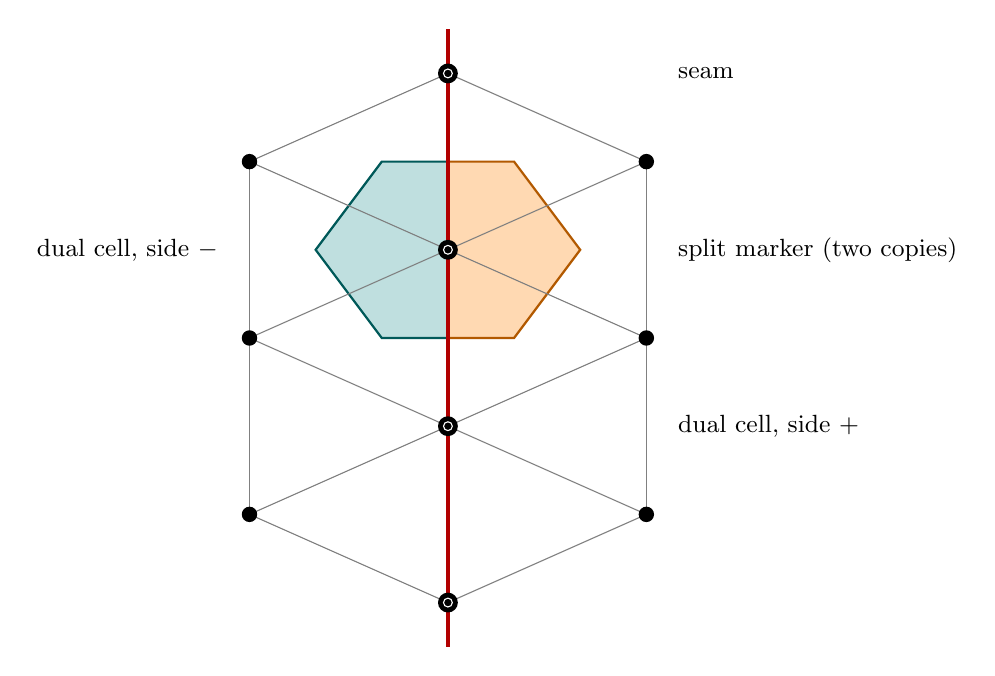
\begin{tikzpicture}[scale=0.028, yscale=-1]
  \fill[teal!25] (200,100)--(170,100)--(155,120)--(140,140)--(155,160)--(170,180)--(200,180)--cycle;
  \fill[orange!30] (200,100)--(230,100)--(245,120)--(260,140)--(245,160)--(230,180)--(200,180)--cycle;
  \draw[teal!70!black,thick] (200,100)--(170,100)--(155,120)--(140,140)--(155,160)--(170,180)--(200,180);
  \draw[orange!70!black,thick] (200,100)--(230,100)--(245,120)--(260,140)--(245,160)--(230,180)--(200,180);
  \draw[gray] (200,60)--(110,100)--(200,140)--(110,180)--(200,220)--(110,260)--(200,300);
  \draw[gray] (110,100)--(110,180)--(110,260);
  \draw[gray] (200,60)--(290,100)--(200,140)--(290,180)--(200,220)--(290,260)--(200,300);
  \draw[gray] (290,100)--(290,180)--(290,260);
  \draw[red!70!black, very thick] (200,40)--(200,320);
  \foreach \p in {(110,100),(110,180),(110,260),(290,100),(290,180),(290,260)} \fill \p circle (3.5);
  \foreach \p in {(200,60),(200,140),(200,220),(200,300)} {\fill \p circle (4.5); \draw[white] \p circle (2);}
  \node[right] at (300,60) {\small seam};
  \node[right] at (300,140) {\small split marker (two copies)};
  \node[left] at (100,140) {\small dual cell, side $-$};
  \node[right] at (300,220) {\small dual cell, side $+$};
\end{tikzpicture}
\caption{A seam (thick line) through the constrained triangulation. The central seam marker has two copies, one per side; each copy's median dual cell is built only from triangles on its own side, so the boundary between the two cells is the seam itself.}
\label{fig:seam}
\end{figure}

\subsection{State variables}
All persistent state is stored per marker copy as integrals over its dual cell:
\begin{equation}
  V_i=\int_{\omega_i}h\dd A,\quad
  M_i=\int_{\omega_i}h\rho_c\dd A,\quad
  Z_i=\int_{\omega_i}\Theta\dd A,\quad
  S_i=\int_{\omega_i}hs\dd A,
\end{equation}
with cell averages $h_i=V_i/A_i$, $\rho_i=M_i/V_i$, $\Theta_i=Z_i/A_i$, $s_i=S_i/V_i$, and column quantities $e_i$, $\Phi_i$ from~\eqref{eq:elev} and~\eqref{eq:phi}. Each subducting-face copy $k$ on a trench additionally stores $W_k$ and $L_k$. Triangles hold no state and may be rebuilt at any time. Rebuilding changes the $A_i$ and hence the cell averages slightly, but never changes any stored integral, so it never changes a budget.

Global budgets are tracked as
\begin{equation}
  \sum_i V_i(t) = \sum_i V_i(0) + V_{\mathrm{created}}(t) - V_{\mathrm{subducted}}(t),
\end{equation}
and likewise for $M$ and $Z$ (for $Z$, with the cooling source added); each side must agree to round-off.

\subsection{Reconstruction}
For a cell-averaged field $f\in\{h,\rho_c,\Theta,s\}$, the linear reconstruction on $\omega_i$ is
\begin{equation}
  f_i(\vect{x}) = f_i + \phi_i\,\vect{G}_i\cdot(\vect{x}-\bar{\vect{x}}_i).
  \label{eq:recon}
\end{equation}
Anchoring the slope at the dual-cell centroid makes the reconstruction conservative: $\int_{\omega_i}f_i(\vect{x})\dd A=f_iA_i$ exactly. The gradient is a weighted least-squares fit over neighbours on the same side of any seam,
\begin{equation}
  \vect{G}_i=\arg\min_{\vect{G}}\sum_j w_{ij}\left(f_j-f_i-\vect{G}\cdot(\bar{\vect{x}}_j-\bar{\vect{x}}_i)\right)^2,
  \qquad w_{ij}=|\bar{\vect{x}}_j-\bar{\vect{x}}_i|^{-2},
\end{equation}
so that reconstructions never smear across plate boundaries. The Barth--Jespersen limiter $\phi_i\in[0,1]$ is the largest value keeping the reconstruction at every segment midpoint of $\omega_i$ within the range of $f$ over $i$ and its neighbours. Setting $\phi_i=0$ gives a robust first-order scheme.

\subsection{Velocity solve}
Velocity is stored at marker copies and interpolated linearly within each triangle (P1 finite elements), so each triangle has constant strain rate. For triangle $c$ with counter-clockwise vertices $(\vect{x}_1,\vect{x}_2,\vect{x}_3)$,
\begin{equation}
  \nabla\varphi_1 = \frac{1}{2A_c}\begin{pmatrix}y_2-y_3\\x_3-x_2\end{pmatrix}\quad\text{and cyclic permutations.}
\end{equation}
In Voigt notation $\boldsymbol\epsilon_c=(\edot_{xx},\edot_{yy},2\edot_{xy})^{\mathsf T}=\mathsf{B}_c\vect{u}_c$, with
\begin{equation}
  \mathsf{B}_c=\begin{pmatrix}
  \partial_x\varphi_1&0&\partial_x\varphi_2&0&\partial_x\varphi_3&0\\
  0&\partial_y\varphi_1&0&\partial_y\varphi_2&0&\partial_y\varphi_3\\
  \partial_y\varphi_1&\partial_x\varphi_1&\partial_y\varphi_2&\partial_x\varphi_2&\partial_y\varphi_3&\partial_x\varphi_3
  \end{pmatrix},
  \qquad
  \mathsf{D}=\begin{pmatrix}2&1&0\\1&2&0\\0&0&\tfrac12\end{pmatrix}.
\end{equation}
Triangle quantities ($h_c$, $\Theta_c$, $s_c$, $\tilde\Phi_c$) are averages of the three vertex values, and $\Hint_c$ follows from~\eqref{eq:visc}. The contributions are:
\begin{align}
  \mathsf{K}_c &= 2A_c\,\Hint_c\,\mathsf{B}_c^{\mathsf T}\mathsf{D}\,\mathsf{B}_c
    &&\text{viscous stiffness ($6\times6$)},\label{eq:Kc}\\
  \vect{F}_{c,a} &= A_c\,\tilde\Phi_c\,\nabla\varphi_a
    &&\text{buoyancy load on vertex $a$},\\
  \mathsf{M}_\beta &= \operatorname{diag}\big(\beta(h_i,\Theta_i)A_i\big)\otimes\vect{I}_2
    &&\text{lumped basal drag}.
\end{align}
The free-edge condition~\eqref{eq:freeedge} with $\Phi_f=\Phi_r$ is the natural boundary condition of this form; it holds on ridge faces with no additional code. A free face whose facing column differs from the ridge column receives the extra traction $(\Phi_r-\Phi_f)\vect{n}$.

\paragraph{Seam terms.} Seam contributions are lumped onto copy pairs. A seam marker with copies $(k^-,k^+)$ has length share $\ell_k$ (half the lengths of its adjacent seam edges), a frame $(\vect{n}_k,\vect{t}_k)$ with $\vect{n}_k$ from side $-$ to side $+$, and coupling tensor $\mathsf{C}_k=C_n\vect{n}_k\vect{n}_k^{\mathsf T}+C_t\vect{t}_k\vect{t}_k^{\mathsf T}$, where $C_n$ is the free or the stiff value according to the pair's contact state (closing or opening, from the current velocity). Coupling adds
\begin{equation}
  \begin{pmatrix}\mathsf{K}_{k^-k^-}&\mathsf{K}_{k^-k^+}\\\mathsf{K}_{k^+k^-}&\mathsf{K}_{k^+k^+}\end{pmatrix}
  \mathrel{+}= \ell_k\begin{pmatrix}\mathsf{C}_k&-\mathsf{C}_k\\-\mathsf{C}_k&\mathsf{C}_k\end{pmatrix},
\end{equation}
which is symmetric positive semi-definite. At a trench, with $k^s$ the subducting and $k^o$ the overriding copy and $\vect{n}_k$ from subducting to overriding, the slab force~\eqref{eq:slabforce} and trench suction add
\begin{equation}
  \vect{F}_{k^s}\mathrel{+}=\ell_kW_k\vect{n}_k,\qquad
  \mathsf{K}_{k^sk^s}\mathrel{+}=\ell_k\,\xi\,\vect{n}_k\vect{n}_k^{\mathsf T},\qquad
  \vect{F}_{k^o}\mathrel{-}=\ell_kP_{ts}\vect{n}_k.
\end{equation}

\paragraph{System.} The assembled system
\begin{equation}
  \big(\mathsf{K}(\vect{u})+\mathsf{M}_\beta\big)\,\vect{u}=\vect{F},
  \label{eq:system}
\end{equation}
with Dirichlet rows eliminated symmetrically, is symmetric positive definite whenever rigid-body modes are removed. Because $\Hint_c$ depends on $\vect{u}$ for $n\ne1$, and the contact state of each seam pair depends on the sign of its normal velocity jump, it is solved by Picard iteration, warm-started from the previous step; contact states are updated from each iterate, as in an active-set method. In the drag-dominated limit it reduces to $\vect{u}\approx-\nabla\Phi/\beta$.

\subsection{Mesh velocity}
Markers move with a velocity $\vect{w}$ that is a free choice. Interior markers use the material velocity plus monitor-weighted smoothing,
\begin{equation}
  \vect{w}_i=\vect{u}_i+\frac{\kappa_m}{\Delta t}\left(\frac{\sum_jm_{ij}\vect{x}_j}{\sum_jm_{ij}}-\vect{x}_i\right),\qquad m_{ij}=\tfrac12(\mathcal{M}_i+\mathcal{M}_j),
  \label{eq:meshvel}
\end{equation}
with relaxation $\kappa_m\in[0,1)$ and monitor $\mathcal{M}_i=1+a_h|\vect{G}^h_i|^2+a_\Theta|\vect{G}^\Theta_i|^2$, or any indicator of where resolution is needed. All copies of a seam marker share one position and so one $\vect{w}$:
\begin{itemize}
\item \textbf{ridge and transform:} the average of the copies' velocities (symmetric spreading), plus tangential smoothing along the chain;
\item \textbf{trench:} the overriding copy's velocity, $\vect{w}_k=\vect{u}_{k^o}$, plus tangential smoothing, so the overriding face is material;
\item \textbf{outer boundary:} normal component material ($\vect{w}\cdot\vect{n}=\vect{u}\cdot\vect{n}$), tangential smoothing only;
\item \textbf{junctions:} the velocity that best satisfies, in least squares, every incident seam's own rule for its normal component (the McKenzie--Morgan construction), falling back to the average over all copies when the seams are parallel.
\end{itemize}

\subsection{Flux update and geometric conservation}
Over a step, markers move linearly, $\vect{x}^{n+1}=\vect{x}^n+\Delta t\,\vect{w}$, so every segment endpoint (a fixed linear combination of marker positions) moves linearly too. Fluxes are evaluated with segment geometry in the midpoint configuration $\vect{x}^{n+1/2}=\vect{x}^n+\tfrac12\Delta t\,\vect{w}$, and with $\vect{v}=\vect{u}-\vect{w}$ interpolated linearly to each segment midpoint.

\paragraph{Internal segments and transform faces.} The volume passing from cell $p$ to cell $q$ is
\begin{equation}
  \Delta V_e=\Delta t\;h^\uparrow(\vect{x}_e)\;\vect{v}_e\cdot\vect{n}_e^{n+1/2}\,|e|^{n+1/2},
  \label{eq:flux}
\end{equation}
where $h^\uparrow$ is the reconstruction~\eqref{eq:recon} of the upwind cell evaluated at the segment midpoint $\vect{x}_e$. For an internal segment the midpoint has barycentric coordinates $(\tfrac5{12},\tfrac5{12},\tfrac16)$ in its triangle. A transform face pairs the two copies across the seam in the same way, so slight convergence or separation exchanges material between plates conservatively. The updates are $V_p\mathrel{-}=\Delta V_e$, $V_q\mathrel{+}=\Delta V_e$, with $M$ and $S$ carried as $\rho_c^\uparrow\Delta V_e$ and $s^\uparrow\Delta V_e$. Because $\Theta$ is per unit area rather than per unit crustal volume, $Z$ has its own flux, $\Delta Z_e=\Delta t\,\Theta^\uparrow(\vect{x}_e)\,\vect{v}_e\cdot\vect{n}_e^{n+1/2}|e|^{n+1/2}$.

\paragraph{Ridge faces.} For a face segment of copy $k$ with outward normal $\vect{n}$ (pointing into the ridge), the plate moves away from the seam when $\vect{v}\cdot\vect{n}<0$, and new lithosphere enters:
\begin{equation}
  \Delta V=\Delta t\,h_{oc}\,(-\vect{v}\cdot\vect{n})_+\,|e|,\quad
  V_k\mathrel{+}=\Delta V,\quad M_k\mathrel{+}=\rho_{oc}\Delta V,\quad S_k\mathrel{+}=\Delta V,\quad Z_k\mathrel{+}=0,
\end{equation}
and $\Delta V$ is added to $V_{\mathrm{created}}$. The face-segment midpoint lies a quarter of the way along the seam edge, so $\vect{v}$ there is $\tfrac34\vect{v}_k+\tfrac14\vect{v}_m$.

\paragraph{Trench faces.} On the subducting face, material leaves when $\vect{v}\cdot\vect{n}>0$:
\begin{equation}
  \Delta V=\Delta t\,h^\uparrow\,(\vect{v}\cdot\vect{n})_+\,|e|,\qquad
  \Delta Z=\Delta t\,\Theta^\uparrow\,(\vect{v}\cdot\vect{n})_+\,|e|,
\end{equation}
removed from the copy (and $M$, $S$ likewise) and added to the subducted budgets. The removed heat deficit feeds the slab reservoir (Section~\ref{sec:sources}). The overriding face is material and carries no flux.

\paragraph{Geometric conservation law.} The area swept by a straight segment whose endpoints move linearly in time has a rate that is linear in time, so the midpoint rule is exact:
\begin{equation}
  A_i^{n+1}-A_i^n=\Delta t\sum_{e\in\partial\omega_i}\vect{w}_e\cdot\vect{n}_e^{n+1/2}|e|^{n+1/2}.
\end{equation}
Hence a uniform state with $\vect{u}=0$ and arbitrary $\vect{w}$ is preserved exactly: moving markers creates no spurious thickness or heat deficit.

\paragraph{Time step.} The update is explicit, with
\begin{equation}
  \Delta t=C\min_i\frac{\sqrt{A_i}}{\max_{e\in\partial\omega_i}|\vect{v}_e|+\epsilon},\qquad C\approx0.4,
\end{equation}
subject also to no cell losing more than its content, no triangle inverting in $\vect{x}^{n+1}$, and $s$ remaining in $[0,1]$; $\Delta t$ is halved if any check fails.

\subsection{Sources}
\label{sec:sources}
After the flux update, cell averages are recomputed with $A_i^{n+1}$ and the local sources applied by operator splitting:
\begin{align}
  \Theta_i &\gets \sqrt{\Theta_i^2+4\kappa\Delta T^2\Delta t/\pi}\;-\;\frac{q_b\,\Delta t}{\rho_mc_p},
  & Z_i&\gets A_i\Theta_i, \label{eq:thsource}\\
  s_i &\gets s_i+\Delta t\,G(s_i,\edot_{E,i}),
  & S_i&\gets V_is_i,
\end{align}
with $\Theta_i$ floored at zero and $\edot_{E,i}$ the area-weighted average over the triangles around $i$. Each subducting copy updates its slab reservoir exactly over the step, with $\Delta Z_k$ the heat deficit it lost to subduction:
\begin{equation}
  W_k\gets W_k\,e^{-\Delta t/\tau_a}+g\rho_m\alpha\,\frac{\Delta Z_k}{\ell_k},\qquad
  L_k\gets L_k+\frac{\Delta V_k}{h_k\,\ell_k}.
\end{equation}
Since $\Delta Z_k/\ell_k=\Theta_{\mathrm{tr}}v_s\Delta t$, this is~\eqref{eq:slab} integrated over the step.

\subsection{Seam events}
\label{sec:events}
The life-cycle conditions of Section~\ref{sec:lifecycle} are evaluated after each step on every seam edge and every interior edge, from the column state of the copies on either side and the velocity jump across the edge. Each edge keeps a persistence clock for its current candidate event. The seams are an explicit set of edges, so a seam may end inside a plate; its tip marker then has a single copy and the seam carries no jump there.
\begin{itemize}
\item \textbf{Nucleation and healing} add or remove seam edges. Markers are then split into copies afresh, one per sector between seam edges. Each old copy's integrals ($V$, $M$, $Z$, $S$, $W\ell$, $L\ell$) go to the new copies in proportion to the corner areas each inherits: healing sums copies, nucleation divides them by dual area, and cell averages are unchanged.
\item \textbf{Changing type} relabels an edge. A new trench starts with an empty reservoir. At breakoff or stall, $W$ and $L$ of the subducting copies are released.
\item \textbf{Trench polarity} is stored per edge relative to the edge's orientation, so that it survives renumbering and changes of plate.
\item \textbf{Plates} are relabelled as the regions seams separate; labels serve only for display and for the coarse space of the solver.
\end{itemize}
Junctions need no special treatment in this bookkeeping: a marker where three or more seams meet simply has three or more copies. They do need it in mesh adaptation, where a sector can shrink to a single sliver triangle.

\subsection{Adaptive insertion and deletion}
\paragraph{Criteria.} A marker is flagged for refinement when $\sqrt{A_i}$ exceeds a fraction of the local feature scale, for example $\sqrt{A_i}|\vect{G}^h_i|/h_i>\tau_r$, $\sqrt{A_i}|\vect{G}^\Theta_i|/\Theta_i>\tau_r$, or $\sqrt{A_i}>\lambda\ell_{d,i}$. It is flagged for coarsening at a smaller threshold $\tau_c<\tau_r$. Neighbouring cell sizes are kept within a factor of about $1.5$, refinement is capped at $A_{\min}$, and seams are kept resolved more finely than the plate interiors around them.

\paragraph{Interior remap.} Inserting a point or deleting a marker changes only the dual cells in a small cavity $\mathcal{C}$. New cell integrals come from intersecting each new cell $\omega'_j$ with each old cell $\omega_i$. Since the reconstruction is linear, the integral over an intersection polygon $P$ needs only its area and centroid:
\begin{equation}
  \int_Pf_i(\vect{x})\dd A=|P|\left(f_i+\phi_i\vect{G}_i\cdot(\bar{\vect{x}}_P-\bar{\vect{x}}_i)\right).
\end{equation}
New cells tile the cavity exactly and each old reconstruction integrates to its old cell integral, so cavity totals are unchanged. Cells are convex, so Sutherland--Hodgman clipping suffices. Insertions must not encroach on seam segments; an encroaching point is replaced by a seam-edge split.

\paragraph{Seam refinement.} Splitting a seam edge inserts a new seam marker with one copy per side; the cavity remap is done separately on each side, so no material crosses the seam. Slab quantities are remapped along the trench by length: $W$ and $L$ are treated as piecewise-constant line densities over each copy's length share, and the total $\sum_kW_k\ell_k$ is preserved.

\subsection{Mesh update: keeping markers on seams without tangling}
\label{sec:meshupdate}
\paragraph{Framing.} Seam segments are triangle edges, and a triangle that never inverts has edges that never cross. So ``the mesh never tangles'' and ``seams never cross'' are one statement, and the mesh update has two parts with separate jobs:
\begin{enumerate}
\item a \emph{move} that never inverts a triangle: $\vect{x}^{n+1}=\vect{x}^n+\Delta t\,\vect{w}$, with $\Delta t$ halved until every triangle stays counter-clockwise (and no cell is drained);
\item a \emph{repair}, between steps, that restores a quality invariant by local, conservative topology changes, so that the next move has room.
\end{enumerate}
Each marker's velocity has a part fixed by physics and a free part. For a seam marker, the normal component is physics (the rules above: mean, overriding copy, or the junction construction); its position \emph{along} the seam is free and is used for smoothing. Interior markers are entirely free; they follow the material to limit numerical diffusion. Repair may change which markers exist and how they are connected, but never moves a marker and never takes a marker off a seam: seam markers are only merged with other seam markers, and seam edges are never flipped, only split or rerouted through a marker already on the seam's path.

\paragraph{Invariant.} Every triangle has all altitudes at least $0.3L_0$ and every edge is shorter than $1.6L_0$, where $L_0$ is the target spacing. Repair inspects every violation by its \emph{thin direction}, a vertex $v$ too close to the opposite edge $ab$ (a short edge is the case $v$ close to $a$ or $b$), and by what $v$ and $ab$ are:
\begin{center}
\begin{tabular}{@{}lll@{}}
\toprule
$v$ & edge $ab$ & operation\\
\midrule
interior & not a seam & flip $ab$ (Delaunay)\\
interior & any & collapse $v$ into $a$ or $b$\\
interior or seam & long ($>1.6L_0$) & split $ab$ (on a seam: one copy per side)\\
on a seam, chain neighbour of $a$ & seam & chain merge: collapse $v$ into $a$ along the seam\\
on a seam, near $a$ & any & zip: collapse $v$ into $a$, merging their seams\\
on a seam, not near an end & seam & snap: flip $ab$ and reroute the seam $a$--$v$--$b$\\
\bottomrule
\end{tabular}
\end{center}
A snap whose flip would invert a triangle falls back to splitting $ab$ at the foot of $v$, followed by a zip. A collapse keeps the endpoint with more seam edges, so junctions survive.

\paragraph{Zip and snap are seam events.} All other operations are numerics. Zip and snap change the seam graph: two seams closer than a cell become one, and the plate sliver between them is gone. This is the resolution limit of the equivalence in Section~\ref{sec:lifecycle}: two seams with a strip narrower than one cell between them are one damaged band, and a damaged band one cell wide is one seam. When two seam edges come to coincide they merge: a trench wins and keeps its polarity, unless the other is a trench of the opposite polarity, in which case the plates on either side now collide and the seam becomes a transform for the life-cycle rules to reclassify; equal types stay; any other pair becomes a transform. Polarity is stored relative to the edge's orientation and survives the move because the side away from the vanished strip is untouched. Two consequences follow without further rules:
\begin{itemize}
\item \emph{Plates can be consumed.} A plate subducting at two converging trenches pinches off where it is narrowest, the trenches zip into one boundary between its former neighbours, and the plate's last slivers are snapped away.
\item \emph{Junctions migrate.} A junction moves along a seam by absorbing the chain marker ahead of it (chain merge, keeping the junction) and, when the wedge between two of its seams closes, by a zip that hands the junction to the marker where the wedge now ends.
\end{itemize}

\paragraph{Remap for seam operations.} A zip or snap moves part of a seam, so area changes sides. The patch's copies are grouped by its triangles, old and new together; since no triangle straddles a seam, each group is one side. Within a group the remap is the interior one. Between groups only net area moves: a group whose area shrank hands that area's worth of its pool, at its own average, to the groups that grew, in proportion to their growth. A copy whose area vanishes hands over everything, and its slab reservoir goes to the largest gainer on its side. Copies are then rebuilt by sector as after seam events. Totals are conserved to round-off and a uniform state stays uniform; the piece that changed sides carries the average of the side it left. This is first order, like the interior remap, and the exact intersection remap applies unchanged.

\paragraph{What is not guaranteed.} An operation can be refused: by the link condition (which keeps the mesh a manifold), by an inverted or too-thin result, or because a surviving copy would be left with almost no area. A refused violation is retried at the next repair. Meanwhile the move shrinks $\Delta t$, and the run stops if $\Delta t$ cannot be made small enough. No bound on refusals is proved.

%======================================================================
\section{Algorithms}
%======================================================================

\begin{algorithm}[H]
\caption{One time step}\label{alg:step}
\begin{algorithmic}[1]
\Require marker copies with $\{\vect{x}_i,V_i,M_i,Z_i,S_i\}$; trench reservoirs $\{W_k,L_k\}$; previous velocity $\vect{u}^{n-1}$
\If{any marker flagged, any seam changed, or mesh quality below threshold}
  \State \Call{Adapt}{} and repair (Section~\ref{sec:meshupdate}): seam splits, chain merges, zips and snaps, interior collapses, splits and flips; assign copies to sectors
\EndIf
\State \Call{Geometry}{} \Comment{Algorithm~\ref{alg:geom}}
\State \Call{ColumnState}{} \Comment{cell averages, limited gradients, $e_i$, $\Phi_i$; Algorithm~\ref{alg:column}}
\State $\vect{u}\gets$ \Call{SolveVelocity}{$\vect{u}^{n-1}$} \Comment{Algorithm~\ref{alg:solve}}
\State $\vect{w}\gets$ mesh velocity by marker type, from~\eqref{eq:meshvel} and the seam rules
\State $\Delta t\gets$ time-step restriction
\State \Call{FluxUpdate}{$\vect{u},\vect{w},\Delta t$} \Comment{Algorithm~\ref{alg:flux}}
\State $\vect{x}_i\gets\vect{x}_i+\Delta t\,\vect{w}_i$
\State \Call{Sources}{$\Delta t$} \Comment{Algorithm~\ref{alg:sources}}
\State \Call{SeamEvents}{$\Delta t$} \Comment{Section~\ref{sec:events}; flags a rebuild if any seam changed}
\State check all budgets to round-off
\end{algorithmic}
\end{algorithm}

\begin{algorithm}[H]
\caption{\textsc{Geometry}: loops over triangles and seam edges}\label{alg:geom}
\begin{algorithmic}[1]
\State $A_i\gets0$, $\bar{\vect{x}}_i\gets\vect{0}$ for all copies
\For{each triangle $c=(a,b,d)$ (copy indices), counter-clockwise}
  \State $A_c\gets$ signed area; abort if $A_c\le0$
  \State basis gradients $\nabla\varphi_a,\nabla\varphi_b,\nabla\varphi_d$; centroid $\vect{g}_c$; edge midpoints
  \For{each vertex $v\in c$ with adjacent midpoints $\vect{m}_1,\vect{m}_2$}
    \State $A_v\mathrel{+}=A_c/3$
    \State $\bar{\vect{x}}_v\mathrel{+}=\frac{A_c}{18}\big[(\vect{x}_v+\vect{m}_1+\vect{g}_c)+(\vect{x}_v+\vect{g}_c+\vect{m}_2)\big]$
  \EndFor
  \State record internal segments $(\vect{g}_c,\vect{m}_{ab}),(\vect{g}_c,\vect{m}_{bd}),(\vect{g}_c,\vect{m}_{da})$ with their cell pairs
\EndFor
\For{each seam edge $km$ and each side}
  \State record face segments $(\vect{x}_k,\vect{m}_{km})$ and $(\vect{m}_{km},\vect{x}_m)$ for the copies on that side
  \State accumulate $\ell_k\mathrel{+}=\tfrac12|km|$, $\ell_m\mathrel{+}=\tfrac12|km|$, and seam normals
\EndFor
\State $\bar{\vect{x}}_i\gets\bar{\vect{x}}_i/A_i$
\end{algorithmic}
\end{algorithm}

\begin{algorithm}[H]
\caption{\textsc{ColumnState}: per-copy column physics}\label{alg:column}
\begin{algorithmic}[1]
\For{each copy $i$}
  \State $h_i\gets V_i/A_i$; $\rho_i\gets M_i/V_i$; $\Theta_i\gets Z_i/A_i$; $s_i\gets S_i/V_i$
  \State $e^\ast\gets e_0+h_i(1-\rho_i/\rho_m)-\alpha\Theta_i$; $e_i\gets e^\ast$ if $e^\ast\ge0$ else $\rho_me^\ast/(\rho_m-\rho_w)$
  \State $\Phi_i\gets$ \eqref{eq:phi}; $\tilde\Phi_i\gets\Phi_i-\Phi_r$
\EndFor
\For{each copy $i$}
  \State least-squares gradients of $h,\rho_c,\Theta,s$ over same-side neighbours; Barth--Jespersen limiters
\EndFor
\end{algorithmic}
\end{algorithm}

\begin{algorithm}[H]
\caption{\textsc{SolveVelocity}: Picard iteration}\label{alg:solve}
\begin{algorithmic}[1]
\Require initial guess $\vect{u}^{(0)}$; tolerance $\delta$; relaxation $\omega\in(0,1]$
\State assemble $\vect{F}$ (buoyancy, free-face, slab, suction terms) and $\mathsf{M}_\beta$ from $\beta(h_i,\Theta_i)$
\State assemble the constant seam terms (tangential coupling, slab drag $\xi$)
\For{$k=0,1,2,\dots$}
  \For{each triangle $c$}
    \State $\boldsymbol\epsilon_c\gets\mathsf{B}_c\vect{u}_c^{(k)}$; $\Hint_c\gets\tfrac12\Bint_c\max(\edot_{E,c},\edot_{\min})^{1/n-1}$
    \State write $2A_c\Hint_c\mathsf{B}_c^{\mathsf T}\mathsf{D}\mathsf{B}_c$ into its matrix slots
  \EndFor
  \For{each seam copy pair $k$}
    \State contact if the normal jump in $\vect{u}^{(k)}$ is one the seam cannot absorb (always, for a transform)
    \State add $\ell_k\mathsf{C}_k$ with stiff or free $C_n$; a pair in contact faces the other side's column, an open ridge pair the ridge column
  \EndFor
  \State solve $(\mathsf{K}+\mathsf{M}_\beta)\vect{u}^\ast=\vect{F}$ with Dirichlet rows eliminated
  \State $\vect{u}^{(k+1)}\gets(1-\omega)\vect{u}^{(k)}+\omega\vect{u}^\ast$
  \If{$\|\vect{u}^{(k+1)}-\vect{u}^{(k)}\|\le\delta\|\vect{u}^{(k+1)}\|$} \Return $\vect{u}^{(k+1)}$ \EndIf
\EndFor
\end{algorithmic}
\end{algorithm}

\begin{algorithm}[H]
\caption{\textsc{FluxUpdate}: conservative ALE transport}\label{alg:flux}
\begin{algorithmic}[1]
\State $\vect{x}^{n+1/2}\gets\vect{x}^n+\tfrac12\Delta t\,\vect{w}$; $\vect{v}\gets\vect{u}-\vect{w}$
\For{each internal segment and each transform face, separating $(p,q)$}
  \State $\vect{n}_e,|e|$ from $\vect{x}^{n+1/2}$; $\vect{v}_e\gets$ interpolate at the segment midpoint
  \State $r\gets p$ if $\vect{v}_e\cdot\vect{n}_e>0$ else $q$
  \State $\Phi^{V}_e\gets\Delta t\,h_r(\vect{x}_e)\,\vect{v}_e\cdot\vect{n}_e|e|$; $\Phi^{Z}_e\gets\Delta t\,\Theta_r(\vect{x}_e)\,\vect{v}_e\cdot\vect{n}_e|e|$
  \State store $(\Phi^V_e,\;\rho_r\Phi^V_e,\;\Phi^Z_e,\;s_r\Phi^V_e)$ in the segment's flux slot
\EndFor
\For{each ridge face segment of copy $k$}
  \State $\Delta V\gets\Delta t\,h_{oc}(-\vect{v}\cdot\vect{n})_+|e|$; store as inflow $(\Delta V,\rho_{oc}\Delta V,0,\Delta V)$; $V_{\mathrm{created}}\mathrel{+}=\Delta V$
\EndFor
\For{each subducting trench face segment of copy $k$}
  \State $\Delta V\gets\Delta t\,h_k(\vect{x}_e)(\vect{v}\cdot\vect{n})_+|e|$; $\Delta Z\gets\Delta t\,\Theta_k(\vect{x}_e)(\vect{v}\cdot\vect{n})_+|e|$
  \State store as outflow; accumulate $\Delta V_k$, $\Delta Z_k$ for the slab; add to subducted budgets
\EndFor
\For{each copy $i$}
  \State add the signed fluxes of its segments and faces to $(V_i,M_i,Z_i,S_i)$, in a fixed order
\EndFor
\end{algorithmic}
\end{algorithm}

\begin{algorithm}[H]
\caption{\textsc{Sources}: thermal, integrity and slab}\label{alg:sources}
\begin{algorithmic}[1]
\For{each copy $i$}
  \State recompute $A_i$ at $\vect{x}^{n+1}$; $\Theta_i\gets Z_i/A_i$; $s_i\gets S_i/V_i$
  \State $\Theta_i\gets\max\!\big(0,\sqrt{\Theta_i^2+4\kappa\Delta T^2\Delta t/\pi}-q_b\Delta t/(\rho_mc_p)\big)$; $Z_i\gets A_i\Theta_i$
  \State $s_i\gets\operatorname{clip}(s_i+\Delta t\,G(s_i,\edot_{E,i}),0,1)$; $S_i\gets V_is_i$
\EndFor
\For{each subducting trench copy $k$}
  \State $W_k\gets W_ke^{-\Delta t/\tau_a}+g\rho_m\alpha\,\Delta Z_k/\ell_k$; $L_k\gets L_k+\Delta V_k/(h_k\ell_k)$
  \If{$L_k>L_{\max}$ and saturation enabled} stop further input to $W_k$ \EndIf
\EndFor
\end{algorithmic}
\end{algorithm}

\begin{algorithm}[H]
\caption{\textsc{Adapt}: conservative insertion and deletion}\label{alg:adapt}
\begin{algorithmic}[1]
\For{each flagged marker (seams first, then interior; refine before coarsen)}
  \If{seam marker or seam edge}
    \State split or merge along the chain; create or remove one copy per side
    \State remap each side's cavity separately; remap $W$, $L$ by length along the trench
  \Else
    \State insert a point (or delete the marker); if the point encroaches a seam, split the seam edge instead
    \State remap the cavity: $V'_j\mathrel{+}=|P|\,h_i(\bar{\vect{x}}_P)$ over $P=\omega'_j\cap\omega_i$, likewise $M'$, $Z'$, $S'$
  \EndIf
  \State assert cavity totals unchanged to round-off
\EndFor
\end{algorithmic}
\end{algorithm}

%======================================================================
\section{Implementation in a web browser with WebGPU}
%======================================================================

\subsection{Division of labour}
Work divides naturally by how often the data's \emph{structure} changes:
\begin{itemize}
\item \textbf{Topology (CPU, JavaScript or WebAssembly):} the CDT, copy-to-sector assignment, adjacency lists, matrix sparsity pattern, and adaptive insertion and deletion. These change only when the mesh is rebuilt, which can be every several steps. Delaunator with Constrainautor provides a constrained Delaunay triangulation in JavaScript; the Triangle library compiled to WebAssembly is an alternative, subject to its licence terms.
\item \textbf{Data-parallel kernels (GPU, WGSL compute shaders):} everything that runs every step with fixed topology, listed in Table~\ref{tab:kernels}.
\item \textbf{Linear solve:} initially on the CPU in double precision (Section~\ref{sec:gpusolve}).
\end{itemize}
Positions stay on the GPU between rebuilds. When the mesh must be rebuilt, positions and state are read back (an asynchronous buffer map), the topology is rebuilt on the CPU, and the new index buffers are uploaded.

\begin{table}[ht]
\centering\small
\begin{tabular}{@{}llll@{}}
\toprule
Kernel & One thread per & Reads & Writes\\
\midrule
Triangle geometry & triangle & positions & $A_c$, $\nabla\varphi$, segment geometry\\
Dual-cell gather & copy & incident triangles & $A_i$, $\bar{\vect{x}}_i$\\
Column state & copy & integrals, $A_i$ & $h,\rho_c,\Theta,s,e,\Phi$\\
Gradients and limiters & copy & neighbour list & $\vect{G}_i$, $\phi_i$\\
Element matrices & triangle & $\vect{u}$, column state & element stiffness, load\\
Matrix gather & matrix nonzero & element entries (gather map) & CSR values\\
Mesh velocity & copy & $\vect{u}$, neighbours, marker type & $\vect{w}$\\
Segment fluxes & segment or face & $\vect{v}$, reconstructions & flux slots\\
Flux gather & copy & incident flux slots & integrals\\
Sources & copy / trench copy & state, $\Delta t$ & $Z,S,W,L$\\
\bottomrule
\end{tabular}
\caption{Per-step compute kernels. Every kernel either writes only to its own thread's outputs or gathers from a precomputed adjacency list.}
\label{tab:kernels}
\end{table}

\subsection{Gather instead of scatter}
Finite element assembly and flux accumulation are naturally scatter operations: each triangle or segment adds into several shared entries. WGSL (the WebGPU Shading Language) provides atomic operations only on 32-bit integers, not on floats. Every scatter is therefore recast as a gather:
\begin{itemize}
\item each triangle or segment writes its contributions to its own slots;
\item a second kernel, one thread per receiving entry (a marker copy or a matrix nonzero), sums the slots listed for it in a compressed sparse row (CSR) adjacency built on the CPU at rebuild time.
\end{itemize}
Summation then happens in a fixed order, so results are reproducible from run to run on the same hardware, and each flux is added to one cell and subtracted from another as the identical floating-point value, which preserves conservation.

\subsection{Precision}
WebGPU provides 32-bit floats in shaders but no 64-bit floats. Three measures keep this from eroding conservation and accuracy:
\begin{enumerate}
\item \textbf{Nondimensionalise} all quantities to order one (lengths by $L_0$, thickness by $h_{oc}$, $\Theta$ by $\Delta T\,h_{oc}$, time by $L_0/U$).
\item \textbf{Store the conserved integrals $V,M,Z,S$ as unevaluated pairs} $(x_{\mathrm{hi}},x_{\mathrm{lo}})$ of 32-bit floats and accumulate fluxes into them with error-free transformations (two-sum). Fluxes themselves are computed in single precision; only accumulation needs the extra bits, because round-off in the state would otherwise grow as a random walk over millions of steps. Verify with a unit test on each target device that the shader compiler preserves the two-sum sequence, since fused or reordered operations would defeat it.
\item \textbf{Check budgets in double precision} on the CPU (JavaScript numbers are 64-bit) at intervals, from read-back state.
\end{enumerate}

\subsection{Linear solver}
\label{sec:gpusolve}
The system~\eqref{eq:system} is symmetric positive definite, but viscosity contrasts between plate interiors and weak boundaries can exceed $10^4$, which makes it ill-conditioned. A staged approach is recommended:
\begin{enumerate}
\item \textbf{Baseline:} assemble values on the GPU, read them back, and solve on the CPU with a double-precision sparse direct solver compiled to WebAssembly. Warm starts are irrelevant for a direct solver, but the factorisation's sparsity analysis can be reused until the next rebuild.
\item \textbf{GPU iterative solve:} preconditioned conjugate gradient (PCG) in single precision, with block-Jacobi ($2\times2$ per marker) preconditioning, warm-started from the previous step's velocity, wrapped in mixed-precision iterative refinement: the residual is computed on the CPU in double precision and the GPU solves only for corrections. Stronger preconditioning, such as algebraic multigrid (AMG), may be needed for large viscosity contrasts.
\end{enumerate}
Profile before moving the solve to the GPU: for meshes up to roughly $10^5$ markers, the CPU direct solve may not be the bottleneck.

\subsection{Buffers, limits and rendering}
\begin{itemize}
\item Use structure-of-arrays storage buffers; allocate with spare capacity so that adaptive changes in marker count rarely force reallocation.
\item Default WebGPU limits allow 65{,}535 workgroups per dispatch dimension; with workgroups of 64 threads, dispatch in two dimensions beyond about four million threads.
\item The marker-position and triangle-index buffers can be bound directly to a render pipeline, so elevation, $\Theta$ or integrity can be drawn every frame without copying data off the GPU.
\end{itemize}

\subsection{Reproducibility}
Record, with every run, all physical and numerical parameters, the mesh-rebuild schedule, the adapter description reported by the browser, and the code version. Maintain a straightforward double-precision reference implementation of every kernel (for example in Python with NumPy) and use it in regression tests that compare GPU output against the reference within stated tolerances. The reference also serves as readable documentation of each kernel.

%======================================================================
\section{Verification}
\label{sec:verification}
%======================================================================
Each test exercises a distinct component and has an exact or algebraic answer.

\paragraph{1. Budgets.} $\sum_iV_i$, $\sum_iM_i$ and $\sum_iZ_i$ must match their budget equations to round-off in every run, including across rebuilds, adaptation, ridge creation and subduction.

\paragraph{2. Free-stream preservation.} Uniform state, $\vect{u}=0$, random smooth $\vect{w}$: all cell averages must stay uniform to round-off.

\paragraph{3. Patch test.} Uniform $h$ and $\Theta$, no drag, cooling disabled, Dirichlet velocities from a linear field $\vect{u}=(ax,by)$ on the boundary: the solution must reproduce the linear field exactly, with $h,\Theta\propto e^{-(a+b)t}$.

\paragraph{4. Drag-dominated spreading.} Uniform $\rho_c$, $\beta$, no thermal contraction, negligible viscosity: continuity becomes the porous medium equation $\partial_th=\tfrac{k}{3}\nabla^2(h^3)$ with $k=g\rho_c(1-\rho_c/\rho_m)/\beta$. With $\tau=kt/3$ its exact solution is
\begin{equation}
  h(r,\tau)=\tau^{-1/3}\left[C-\frac{r^2}{18}\tau^{-1/3}\right]_+^{1/2},\qquad C=\left(\frac{V_{\mathrm{tot}}}{12\pi}\right)^{2/3}.
\end{equation}

\paragraph{5. Steady ridge.} A rigid plate spreading at prescribed rate $U$ from a ridge: $\Theta$ must equal $2\Delta T\sqrt{\kappa x/(\pi U)}$ at distance $x$, depth must follow $e_r-\rho_m\alpha\Theta/(\rho_m-\rho_w)$, and the depth-integrated stress transmitted at age $\tau$ must match~\eqref{eq:ridgepush}.

\paragraph{6. Transform.} Two plates sliding past each other along a transform: normal opening must vanish as $C_n$ increases, with tangential slip governed by $C_t$.

\paragraph{7. Slab feedback.} A nearly rigid plate of area $A_p$ with trench length $\ell_{\mathrm{tr}}$, uniform drag and ridge push $F_{rp}$ per unit ridge length $\ell_r$. In steady state, $W=\tau_ag\rho_m\alpha\Theta_{\mathrm{tr}}v$, and force balance gives
\begin{equation}
  v\left(\beta A_p+\xi\ell_{\mathrm{tr}}-\tau_ag\rho_m\alpha\Theta_{\mathrm{tr}}\ell_{\mathrm{tr}}\right)=F_{rp}\ell_r,
\end{equation}
so the plate reaches the terminal velocity this predicts when $\Gamma<1$, and accelerates without bound otherwise. Both regimes should be reproduced, and the approach to steady state should take a few $\tau_a$.

\paragraph{8. Seam events.} Budgets close to round-off across every nucleation, healing and relabelling, and a uniform state stays uniform when copies are split or merged. Scenarios check each rule: an idle transform heals; a seamless sheet under sustained shear nucleates transforms along the shear zone; a transform pushed shut between old and young lithosphere becomes a trench with the old side subducting; a transform pulled apart opens a ridge in thin lithosphere but not in thick; a ridge pushed shut becomes a transform; and a plate carrying a continent into a trench loses its slab when the continent arrives. Without an external push the plate then decelerates over a few $\tau_a$; with one, subduction may restart with the opposite polarity.

\paragraph{9. Sensitivity.} Features reported as results must persist under resolution refinement, rebuild frequency, mesh-velocity parameters, adaptation thresholds, seam-event thresholds and persistence times, and comparison of GPU and reference implementations.

\paragraph{10. Mesh update.} Prescribed rigid rotations (no solve), so that the geometry is known. A plate subducting at two trenches whose overriding plates converge on it must be consumed at the time the rates predict, with its two trenches zipping into one boundary between its neighbours, budgets closing to round-off, and a uniform state staying uniform through every zip and snap. Splitting seam edges must conserve integrals and slab reservoirs to round-off and keep every trench's polarity.

%======================================================================
\section{Status of the components}
%======================================================================
\begin{center}
\begin{tabular}{@{}p{0.42\textwidth}p{0.52\textwidth}@{}}
\toprule
Component & Status\\
\midrule
Thin viscous sheet with GPE forcing & Established\\
Half-space cooling, depth $\propto\sqrt{\text{age}}$, ridge push~\eqref{eq:ridgepush} & Established\\
Heat-deficit closure~\eqref{eq:cooling} & Exact for half-space cooling under depth-uniform strain; the basal-flux term is a modelling choice\\
Linear finite elements, vertex-centred finite volumes, CDT, split-node seams & Standard techniques\\
Exact conservation and geometric conservation & Exact by construction; verified by tests 1--2\\
Mesh velocity and adaptation criteria & Method choices affecting accuracy, not conservation\\
Zip and snap (seams closer than a cell merge) & Modelling choice at the resolution limit: the merge rule for seam types; the timing is mesh-dependent\\
Integrity law, strength coefficients $B_c$, $B_l$ & Modelling choices requiring physical justification\\
Slab reservoir ($\tau_a$, $\xi$, $L_{\max}$) & Modelling choice; calibrate against observed plate speeds and their correlation with trench length\\
Strain localisation with damage & Mesh-dependent unless $G$ contains a physical length scale; adaptivity amplifies this\\
Seam life cycle (nucleation, conversion, breakoff, healing) & Modelling choice: switches between equivalent descriptions (seam $\leftrightarrow$ damaged band), with persistence times and hysteresis; nucleation is mesh-dependent, seam damage uses the physical fault-zone width $w_f$\\
Thickness-dependent basal drag & Modelling choice; constrain $c_k$ and $m$ by the observed slowness of plates with large continental keels\\
Planar geometry & Global models require markers on a sphere (whose convex hull is the Delaunay triangulation) with per-triangle tangent frames; flat triangles on a sphere then satisfy the geometric conservation law only approximately\\
\bottomrule
\end{tabular}
\end{center}

\begin{thebibliography}{99}
\bibitem{em82} P.~England and D.~McKenzie, A thin viscous sheet model for continental deformation, \emph{Geophys.\ J.\ R.\ Astron.\ Soc.} \textbf{70} (1982) 295--321.
\bibitem{he86} G.~A.~Houseman and P.~England, Finite strain calculations of continental deformation 1: Method and general results for convergent zones, \emph{J.\ Geophys.\ Res.} \textbf{91} (1986) 3651--3663.
\bibitem{ml88} P.~Molnar and H.~Lyon-Caen, Some simple physical aspects of the support, structure, and evolution of mountain belts, \emph{Geol.\ Soc.\ Am.\ Spec.\ Pap.} \textbf{218} (1988) 179--207.
\bibitem{ts} D.~L.~Turcotte and G.~Schubert, \emph{Geodynamics}, Cambridge University Press.
\bibitem{ps77} B.~Parsons and J.~G.~Sclater, An analysis of the variation of ocean floor bathymetry and heat flow with age, \emph{J.\ Geophys.\ Res.} \textbf{82} (1977) 803--827.
\bibitem{mck78} D.~McKenzie, Some remarks on the development of sedimentary basins, \emph{Earth Planet.\ Sci.\ Lett.} \textbf{40} (1978) 25--32.
\bibitem{good58} T.~R.~Goodman, The heat-balance integral and its application to problems involving a change of phase, \emph{Trans.\ ASME} \textbf{80} (1958) 335--342.
\bibitem{fu75} D.~Forsyth and S.~Uyeda, On the relative importance of the driving forces of plate motion, \emph{Geophys.\ J.\ R.\ Astron.\ Soc.} \textbf{43} (1975) 163--200.
\bibitem{mr81} H.~J.~Melosh and A.~Raefsky, A simple and efficient method for introducing faults into finite element computations, \emph{Bull.\ Seismol.\ Soc.\ Am.} \textbf{71} (1981) 1391--1400.
\bibitem{sh96} J.~R.~Shewchuk, Triangle: engineering a 2D quality mesh generator and Delaunay triangulator, in \emph{Applied Computational Geometry}, Lecture Notes in Computer Science \textbf{1148} (1996) 203--222.
\bibitem{bp80} B.~R.~Baliga and S.~V.~Patankar, A new finite-element formulation for convection-diffusion problems, \emph{Numer.\ Heat Transfer} \textbf{3} (1980) 393--409.
\bibitem{tl79} P.~D.~Thomas and C.~K.~Lombard, Geometric conservation law and its application to flow computations on moving grids, \emph{AIAA J.} \textbf{17} (1979) 1030--1037.
\bibitem{bj89} T.~J.~Barth and D.~C.~Jespersen, The design and application of upwind schemes on unstructured meshes, AIAA Paper 89-0366 (1989).
\bibitem{mac89} D.~R.~MacAyeal, Large-scale ice flow over a viscous basal sediment: theory and application to Ice Stream B, Antarctica, \emph{J.\ Geophys.\ Res.} \textbf{94} (1989) 4071--4087.
\bibitem{vaz07} J.~L.~V\'azquez, \emph{The Porous Medium Equation: Mathematical Theory}, Oxford University Press (2007).
\bibitem{ber03} D.~Bercovici, The generation of plate tectonics from mantle convection, \emph{Earth Planet.\ Sci.\ Lett.} \textbf{205} (2003) 107--121.
\end{thebibliography}

\end{document}
